\documentclass[../main.tex]{subfiles}

\begin{document}

\chapter{Matrices}

Matrices are one of the fundamental components that build linear
algebra. This note discusses the fundamental concepts and properties
of matrices.

\section{Basic Terms and Notations}

As always, let's get started with the definition.

\begin{definition}
A \textbf{matrix} is a 2-dimensional array composed of entries
called \textbf{elements}. A matrix is said to have \textbf{order}
``$m$ by $n$'' and written as $m \times n$ if there are $m$ rows
and $n$ columns.
\end{definition}

Technically, the elements of a matrix can be anything including
functions. However, the majority of the matrices discussed in
linear algebra will have numeric elements. Let's take a look
at some examples.
\[
A=
\begin{bNiceMatrix}[last-row,last-col]
    1  &  2 &  3 & 4  &
        \Vbrace[horizontal-label]{3}{3 \text{ rows}} \\
    -1 & -2 & -3 & -4 \\
    0  & -1 & 0  & 1  \\
    \Hbrace{4}{4 \text{ columns}} &
\end{bNiceMatrix}
\qquad\quad,\qquad
B =
\begin{bNiceMatrix}[last-row,last-col]
\pi & \Vbrace[horizontal-label]{4}{4 \text{ rows}} \\
e \\
0 \\
1 \\
\Hbrace{1}{1 \text{ column}}
\end{bNiceMatrix}
\]
Here, matrix $A$ has order $3 \times 4$ and matrix $B$ has
order $4 \times 1$. The form of a matrix that has order
$m \times n$ can be generalized as the following.
\[
A=
\begin{bNiceMatrix}[last-row,last-col]
    a_{1,1} & a_{1,2} & a_{1,3} & \cdots & a_{1,n}
        & \Vbrace[horizontal-label]{5}{n \text{ rows}} \\
    a_{2,1} & a_{2,2} & a_{2,3} & \cdots & a_{2,n} \\
    a_{3,1} & a_{3,2} & a_{3,3} & \cdots & a_{3,n} \\
    \vdots  & \vdots  & \vdots  & \ddots & \vdots  \\
    a_{m,1} & a_{m,2} & a_{m,3} & \cdots & a_{m,n} \\
    \Hbrace{5}{m \text{ columns}} &
\end{bNiceMatrix}
\]
It is also worth noting that matrix $A$ is often represented
as $[a_{ij}]$ and the elements as $a_{ij}$ like $a_{12}$ for
$a_{1, 2}$.

\begin{definition}
An element $a_{ij}$ is said to have row index of $i$ and
column index of $j$.
\end{definition}

As you probably have guessed, we assign special names to some
matrices depending on $m$ and $n$.

\begin{definition}
\textbf{Square matrices} are matrices with an equal number of rows
and columns. The elements with the same row and column index are
called \textbf{diagonal elements} of the matrix. The collection
of such elements is called \textbf{main diagonal}, or
\textbf{principal diagonal}.
\end{definition}

What if either $m$ or $n$ is equal to $1$? Yes, we do have special
terms for them.

\begin{definition}
\textbf{Row matrices} are matrices that are composed of only one
row. A \textbf{column matrix} is an array composed of one column.
\end{definition}

If you have a machine learning background, you likely have heard
of the term ``high dimensional arrays or vectors.'' Here, the
term ``dimension'' works the same way.

\begin{definition}
The \textbf{dimension} of a row or column matrix is the number
of \textbf{components}, or the elements. An
\textbf{$\mathbf{n}$-tuple} is an $n$-dimensional row or column
vector.
\end{definition}

Let's take a look at an example from the previous matrix $B$
reproduced below.

\begin{minipage}{0.2\textwidth}
\[
B =
\begin{bNiceMatrix}[last-row,last-col]
\pi & \Vbrace[horizontal-label]{4}{4 \text{ rows}} \\
e \\
0 \\
1 \\
\Hbrace{1}{1 \text{ column}}
\end{bNiceMatrix}
\]
\end{minipage}
\hfill
\begin{minipage}{0.7\textwidth}
Here, matrix $B$ is a 4-dimensional matrix with four components.
This column matrix can also be called as $4$-tuple.
\end{minipage}

We could also define matrices by their elements.

\begin{definition}
A \textbf{zero matrix} is a matrix with all its elements as $0$.
\end{definition}

With the fundamental terms in mind, let's discuss the properties
of matrices.

\section{Fundamental Properties}

First, when are two matrices ``equal'' to each other? Consider
the following definition for a formal explanation.

\begin{theorem}{Equality of Matrix}
Two matrices $A$ and $B$ with orders $m \times n$ and $p \times q$
respectively are said to be equal to each other if they retain
the same order and corresponding elements, i.e. they satisfy the
following properties.
\begin{enumerate}
\item $m = p$
\item $n = q$
\item
For elements $a_{ij}$ in $A$ and $b_{ij}$ in $B$, the following
equation satisfies.
\[
a_{ij} = b_{ij} \,
    \forall \, i \in [1, m] \text{ and } j \in [1, n]
\]
\end{enumerate}
\end{theorem}

Although this is very trivial and intuitive, it is always nice
to formally define concepts!

\begin{theorem}{Matrix Addition}
For matrices $A$ and $B$ with same order, the element in the
$(i, j)$-entry of their sum $A + B$ is equivalent to the sum of
elements in the $(i, j)$-entry of $A$ and $B$.
\end{theorem}

Note that the orders of matrices being added must be identical.
We do not consider additions with matrices of different orders.
Below is an example of addition.
\[
\begin{bmatrix}
    1 & 3   & 5 \\
    2 & \pi & 4
\end{bmatrix}
+
\begin{bmatrix}
    -2 & 1   & 3 \\
    3  & \pi & -4
\end{bmatrix}
=
\begin{bmatrix}
    -1 & 4    & 8 \\
    5  & 2\pi & 0
\end{bmatrix}
\]
Similarly, we could see that subtractions are defined in similar
way. Subtracting the matrices above, we get the following results.
\[
\begin{bmatrix}
    1 & 3   & 5 \\
    2 & \pi & 4
\end{bmatrix}
-
\begin{bmatrix}
    -2 & 1   & 3 \\
    3  & \pi & -4
\end{bmatrix}
=
\begin{bmatrix}
    3  & 2 & 2 \\
    -1 & 0 & 8
\end{bmatrix}
\]
Now, as we look at the additions and subtractions of matrices,
you probably wondered about the application of additive properties.
Intuitively, the fundamental properties of addition can be
applied to matrices addition.

\begin{theorem}{Commutative Property of Matrix Addition}
For matrices $A$ and $B$ with order $m \times n$, $A + B = B + A$.
\end{theorem}
\begin{proof}
Let $A = [a_{ij}]_{m \times n}$ and $B = [b_{ij}]_{m \times n}$.
By definition, the sum $A + B = [a_{ij} + b_{ij}]$. Because
addition is commutative, the following equation holds.
\[
A + B
= [a_{ij} + b_{ij}]
= [b_{ij} + a_{ij}]
= B + A
\]
Thus, the commutative property of matrix addition holds.
\end{proof}

In addition to the commutative property, the associative property
is also applicable.

\begin{theorem}{Associative Property of Matrix Addition}
For matrices $A$, $B$, and $C$ with order $m \times n$,
$A + (B + C) = (A + B) + C$.
\end{theorem}
\begin{proof}
Let $A = [a_{ij}]_{m \times n}$, $B = [b_{ij}]_{m \times n}$,
and $C = [c_{ij}]_{m \times n}$. Consider the following equation.
\begin{align*}
    A + (B + C)
    &= [a_{ij}] + [b_{ij} + c_{ij}]
     = [a_{ij} + (b_{ij} + c_{ij})]
     = [a_{ij} + b_{ij} + c_{ij}] \\
    &= [(a_{ij} + b_{ij}) + c_{ij}]
     = [a_{ij} + b_{ij}] + [c_{ij}] \\
    &= (A + B) + C
\end{align*}
Thus, the associative property of addition applies to the matrix
addition.
\end{proof}

One obvious property in addition is that when you add $0$ to a number,
you get the number itself. The same applies in matrix addition.

\begin{theorem}{Additive Identity of Matrix Addition}
The sum of matrices $A_{m \times n}$ and $0_{m \times n}$ yields
the matrix $A$, i.e. the zero matrix is the identity elements of
matrix addition.
\end{theorem}
\begin{proof}
Let $A = [a_{ij}]_{m \times n}$. By definition, the sum $A + 0
= [a_{ij} + 0] = [a_{ij}] = A$. Therefore, the zero matrix is the
identity element of matrix addition.
\end{proof}

Now what if we want to add the same matrix multiple times?
Fortunately, we already resolved the issue. For instance,
we write $x + x + x$ as $3x$. We can multiply matrices with scalars.

\begin{theorem}{Scalar Multiplication}
For a complex number $\lambda$ and $A = [a_{ij}]$, $\lambda A
= [\lambda a_{ij}]$.
\end{theorem}

Let's take a look at an example.

\begin{problem}
Compute $2A - 3B$ for $A$ and $B$ defined as the following.
\[
A =
\begin{bmatrix}
    2 & 3 & -1 \\
    1 & 7 & 3
\end{bmatrix},
\quad
B =
\begin{bmatrix}
    -2 & 1 & 0 \\
    5  & 3 & 8
\end{bmatrix}
\]
\end{problem}
\begin{solution}
Before subtracting, we could perform scalar multiplication first.
\begin{align*}
2A - 3B
&=
2\begin{bmatrix}
    2 & 3 & -1 \\
    1 & 7 & 3
\end{bmatrix}
-
3\begin{bmatrix}
    -2 & 1 & 0 \\
    5  & 3 & 8
\end{bmatrix} \\
&=
\begin{bmatrix}
    4 & 6  & -2 \\
    2 & 14 & 6
\end{bmatrix}
-
\begin{bmatrix}
    -6 & 3 & 0 \\
    15 & 9 & 24
\end{bmatrix}
\end{align*}
From here we could subtract two matrices. Therefore, $2A - 3B$
can be represented as following.
\[
2A - 3B =
\begin{bmatrix}
    10  & 3  & -2 \\
    -13 & 5 & -18
\end{bmatrix}
\]
\end{solution}

With the scalar multiplication in mind, we can expand the application
of foundational concepts here with matrices.

\begin{theorem}{Additional Properties}
For $A = [a_{ij}]_{m \times n}$, $B = [b_{ij}]_{m \times n}$,
and $\lambda_1, \lambda_2 \in \mathbb{C}$, the following
properties hold.
\begin{enumerate}
\item $\lambda_1 (A \pm B) = \lambda_1 A \pm \lambda_1 B$
\item $(\lambda_1 \pm \lambda_2) A = \lambda_1 A \pm \lambda_2 A$
\item $\lambda_1 (\lambda_2 A) = (\lambda_1 \lambda_2) A$
\end{enumerate}
\end{theorem}

Let's prove them! Below is the proof for the first property.

\begin{proof}
Consider the following equation.
\[
\lambda_1 (A \pm B)
= \lambda_1 ([a_{ij}] \pm [b_{ij}])
= \lambda_1 ([a_{ij} \pm b_{ij}])
\]
Note that individual elements are multiplied in scalar multiplication.
Moreover, because $\lambda_1 (a_{ij} \pm b_{ij}) = \lambda_1 a_{ij}
\pm \lambda_1 b_{ij}$, the following equation holds.
\[
\lambda_1 ([a_{ij} \pm b_{ij}])
= [\lambda_1 a_{ij} \pm \lambda_1 b_{ij}]
= [\lambda_1 a_{ij}] \pm [\lambda_1 b_{ij}]
= \lambda_1 A \pm \lambda_1 B
\]
Therefore, $\lambda_1 (A \pm B) = \lambda_1 A \pm \lambda_1 B$.
\end{proof}

Now let's prove the second property.

\begin{proof}
By definition of scalar multiplication, $(\lambda_1 \pm \lambda_2)
A$ can be represented as the following.
\[
(\lambda_1 \pm \lambda_2) A
= (\lambda_1 \pm \lambda_2) [a_{ij}]
= [(\lambda_1 \pm \lambda_2) a_{ij}]
\]
Using the distributive property, the following equation holds.
\[
[(\lambda_1 \pm \lambda_2) a_{ij}]
= [\lambda_1 a_{ij} \pm \lambda_2 a_{ij}]
= [\lambda_1 a_{ij}] \pm [\lambda_2 a_{ij}]
= \lambda_1 A \pm \lambda_2 A
\]
Thus, the equation $(\lambda_1 \pm \lambda_2) A =
\lambda_1 A \pm \lambda_2 A$ holds.
\end{proof}

Finally, here is the proof to the third property.

\begin{proof}
Consider the following equation.
\begin{align*}
    \lambda_1 (\lambda_2 [a_{ij}])
    &= \lambda_1 [\lambda_2 a_{ij}]
    = [\lambda_1 \lambda_2 a_{ij}]
    = [(\lambda_1 \lambda_2) a_{ij}] \\
    &= (\lambda_1 \lambda_2) [a_{ij}]
    = (\lambda_1 \lambda_2) A
\end{align*}
Therefore, the property holds.
\end{proof}

We have discussed fundamental properties so far. In the next
section of the note, let's discuss what matrix multiplication
with intuitions and computations.

\section{Matrix Multiplication}

Before we get into formulas and computations, let's build our
intuition on what a matrix and its multiplication is supposed to
represent. We will discuss \textbf{linear transformation} in
depth in latter notes, but we can think of it as a function that
transforms the vector space. Matrix instructs the function how to
transform the space. Let's take a look at a quick example.

Let $A$ be a matrix that has order $2 \times 2$. The first column
tells how to map the $\hat{i}$ and the second column represents
where our $\hat{j}$ is mapped.
\[
\begin{bmatrix}
    2 & 1 \\
    1 & 3
\end{bmatrix}
\]
Matrix $A$ is telling us to map the standard basis $\hat{i} =
\langle 1, 0 \rangle$ to $\hat{i}'= \langle 2, 1 \rangle$ and from
$\hat{j} = \langle 0, 1 \rangle$ to $\hat{j}' = \langle 1, 3 \rangle$.
Consider the diagram below.

\begin{figure}[H]
\centering
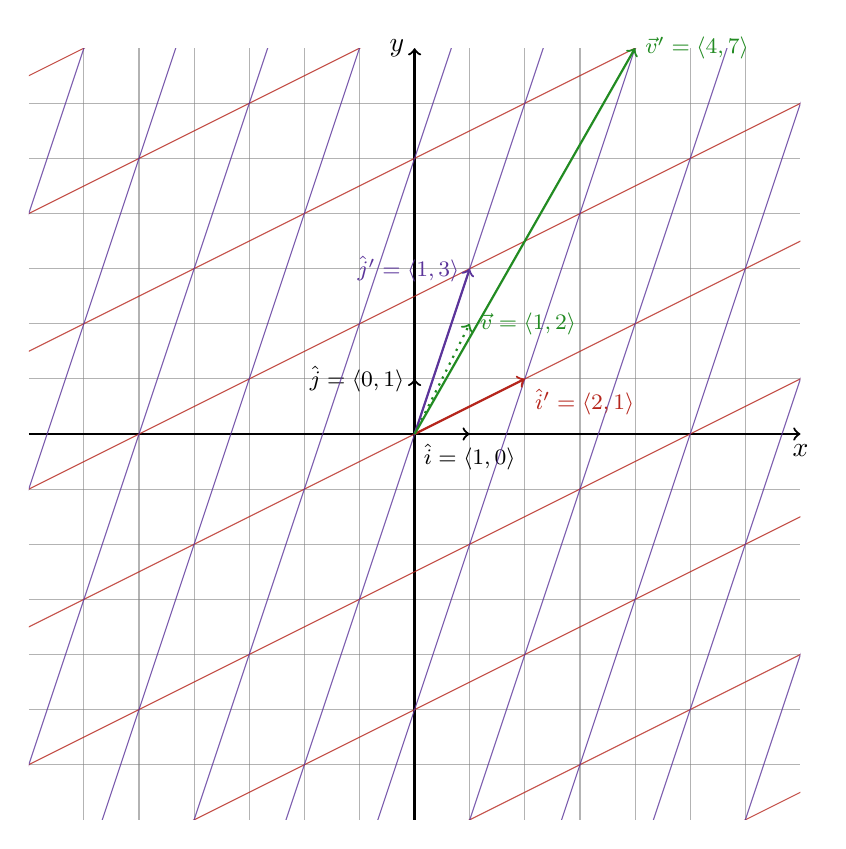
\begin{tikzpicture}[
        vector/.style={->, thick},
        scale=0.7
    ]

    \foreach \i in {-6, -5, ..., 6} {
        \draw[gray, thin, opacity=0.6] (\i, -7) -- (\i, 7);
        \draw[gray, thin, opacity=0.6] (-7, \i) -- (7, \i);
    }
    \draw[vector, black] (-7, 0) -- (7, 0) node[below] {$x$};
    \draw[vector, black] (0, -7) -- (0, 7) node[left] {$y$};

    \draw[vector] (0, 0) -- (1, 0) node[below]
        {\footnotesize $\hat{i} = \langle 1, 0 \rangle$};
    \draw[vector] (0, 0) -- (0, 1) node[left]
        {\footnotesize $\hat{j} = \langle 0, 1 \rangle$};
    \draw[vector, dotted, ForestGreen] (0, 0) -- (1, 2)
        node[right, ForestGreen]
            {\footnotesize $\vec{v} = \langle 1, 2 \rangle$};

    \begin{scope}
        \clip (-7, -7) rectangle (7, 7);

        \foreach \j in {-10, -9, ..., 10} {
            \draw[BrickRed, opacity=0.8]
                ({-10*2 + \j*1}, {-10*1 + \j*3})
                    -- ({10*2 + \j*1}, {10*1 + \j*3});
        }
        \foreach \i in {-10, -9, ..., 10} {
            \draw[RoyalPurple, opacity=0.8]
                ({\i*2 + -10*1}, {\i*1 + -10*3})
                    -- ({\i*2 + 10*1}, {\i*1 + 10*3});
        }
    \end{scope}

    \draw[vector, BrickRed] (0, 0) -- (2, 1)
        node[below right, BrickRed]
            {\footnotesize $\hat{i}' = \langle 2, 1 \rangle$};
    \draw[vector, RoyalPurple] (0, 0) -- (1, 3)
        node[left, RoyalPurple]
            {\footnotesize $\hat{j}' = \langle 1, 3 \rangle$};
    \draw[vector, ForestGreen] (0, 0) -- (4, 7)
        node[right, ForestGreen]
            {\footnotesize $\vec{v}' = \langle 4, 7 \rangle$};
\end{tikzpicture}
\end{figure}

After the transformation, you can imagine mapping everything
in the standard vector space with respect to the new colored
space. That, is what matrix multiplication does. See how
a vector $\vec{v} = \langle 1, 2 \rangle$ is now on
$\langle 4, 7 \rangle$. Using matrix multiplication, we can
represent the mapping as the following.
\[
\begin{bmatrix}
    2 & 1 \\
    1 & 3
\end{bmatrix}
\begin{bmatrix}
    1 \\
    2
\end{bmatrix}
=
\begin{bmatrix}
    4 \\
    7
\end{bmatrix}
\]
Because we cannot draw such planes every time, let's take a look
at how the vector $\vec{v} = \langle 1, 2 \rangle$ is mapped to
$\langle 4, 7 \rangle$. First, from the previous note, we have seen
that the first row represents the $x$ coordinate and the second
row represents the $y$ coordinate. Now, to find where the point
$(1, 2)$ is located in the ``scaled'' version, we could simply look
at the basis vectors in the ``scaled'' plane. Because the vector
that we are looking for is the sum of the two ``scaled'' basis
vector, we can represent our multiplication as the following.
\[
\begin{bmatrix}
    2 & 1 \\
    1 & 3
\end{bmatrix}
\begin{bmatrix}
    1 \\
    2
\end{bmatrix}
=
1
\begin{bmatrix}
    2 \\
    1
\end{bmatrix}
+
2
\begin{bmatrix}
    1 \\
    3
\end{bmatrix}
=
\begin{bmatrix}
    2 \\
    1
\end{bmatrix}
+
\begin{bmatrix}
    2 \\
    6
\end{bmatrix}
=
\begin{bmatrix}
    4 \\
    7
\end{bmatrix}
\]
Nice! We get the same result. Now that we have intuitions on what
a matrix and its multiplication represents, let's take a look at
algebraic properties and resulting formulas from the intuition.

\subsection{The Method and Properties}

As you can see above, matrix multiplication is not defined
elementwise unlike addition and scalar multiplication. First,
take a look at the following formula for individual elements.

\begin{theorem}{Matrix Multiplication}
For matrices $[a_{ij}]_{m \times n}$ and $[b_{ij}]_{n \times p}$,
the elements $c_{ij}$ of the product matrix $[c_{ij}]_{m \times p}$
are defined as the following expression.
\[
c_{ij}
= \sum_{k=1}^{n} a_{ik} b_{kj}
\]
\end{theorem}

Let's take a look at an example to see how this works.

\begin{problem}
Compute the following matrix multiplication.
\[
\begin{bmatrix}
    2 & 3 & 4 \\
    1 & 5 & -1
\end{bmatrix}
\begin{bmatrix}
    1 & 2 \\
    2 & 3 \\
    4 & 0
\end{bmatrix}
\]
\end{problem}
\begin{solution}
Consider the following computation.
\begin{align*}
\begin{bmatrix}
    \tikzmarknode{a11}{2} &
    \tikzmarknode{a12}{3} &
    \tikzmarknode{a13}{4} \\
    \tikzmarknode{a21}{1} &
    \tikzmarknode{a22}{5} &
    \tikzmarknode{a23}{-1}
\end{bmatrix}
\begin{bmatrix}
    \tikzmarknode{b11}{1} &
    \tikzmarknode{b12}{2} \\
    \tikzmarknode{b21}{2} &
    \tikzmarknode{b22}{3} \\
    \tikzmarknode{b31}{4} &
    \tikzmarknode{b32}{0}
\end{bmatrix}
\begin{tikzpicture}[
        overlay, remember picture,
        arrow/.style = {->, very thick, opacity=0.7}
    ]
    \draw[arrow, Red] (a11.west) -- (a13.east);
    \draw[arrow, Blue] (a21.west) -- (a23.east);
    \draw[arrow, Red] (b11.north west) -- (b31.south west);
    \draw[arrow, Blue] (b11.north east) -- (b31.south east);
    \draw[arrow, Red] (b12.north west) -- (b32.south west);
    \draw[arrow, Blue] (b12.north east) -- (b32.south east);
\end{tikzpicture}
&=
\begin{bmatrix}
    \textcolor{Red}{2} \cdot 1 +
    \textcolor{Red}{3} \cdot 2 +
    \textcolor{Red}{4} \cdot 4 &
    \textcolor{Red}{2} \cdot 2 +
    \textcolor{Red}{3} \cdot 3 +
    \textcolor{Red}{4} \cdot 0 \\
    \textcolor{Blue}{1} \cdot 1 +
    \textcolor{Blue}{5} \cdot 2 -
    \textcolor{Blue}{1} \cdot 4 &
    \textcolor{Blue}{1} \cdot 2 +
    \textcolor{Blue}{5} \cdot 3 -
    \textcolor{Blue}{1} \cdot 0
\end{bmatrix} \\
&=
\begin{bmatrix}
    2 + 6 + 16 &
    4 + 9 + 0 \\
    1 + 10 - 4 &
    2 + 15
\end{bmatrix}
=
\begin{bmatrix}
    24 & 13 \\
    7 & 17
\end{bmatrix}
\end{align*}
\end{solution}

It is important to note that matrix multiplication applies under
a specific condition.

\begin{theorem}{Condition for Matrix Multiplication}
For matrices $A_{m \times n}$ and $B_{p \times q}$, the matrices
can be multiplied if and only if $n = p$. The resulting matrix
will have order $m \times q$.
\end{theorem}

I believe the condition above is somewhat self-evident. When the
condition above is not met, we say the product is \textbf{undefined}.
Continuing from this condition, we could get an interesting property.

\begin{theorem}{Commutativity of Matrix Multiplication}
Matrix multiplication is not commutative, i.e. for matrices $A$ and
$B$, it is not necessarily true that $AB = BA$.
\end{theorem}
\begin{proof}
I will leave a more formal proof for the readers. However, I believe
this is self-evident as for matrices $A_{m \times n}$ and
$B_{n \times p}$ where $m \neq p$, $AB$ is defined while $BA$ is not.
\end{proof}

A fun way of understanding commutativity is to think about
transformation questions that we see in elementary or middle school
competition math. You might be familiar with questions asking orders
of transformation of an object. For instance, let $A$ be defined
as the $90^\circ$ rotation counterclockwise and let transformation
$B$ be reflection across the $y$ axis. Is performing $AB$ equal to
$BA$? Obviously, the answer is false when you visually think about it.
What if we apply the same idea here with matrices?

Notice the matrices $A$ and $B$ can be represented as following using
matrices.
\[
A =
\begin{bmatrix}
    0 & -1 \\
    1 & 0
\end{bmatrix},
\quad
B =
\begin{bmatrix}
    -1 & 0 \\
    0  & 1
\end{bmatrix}
\]
Taking a look at the visualization, the left diagram represents
$AB$ and the right diagram visualizes $BA$ with $\vec{v} =
\langle 1, 1 \rangle$ as the reference.

\begin{minipage}{0.48\textwidth}
\begin{figure}[H]
\centering
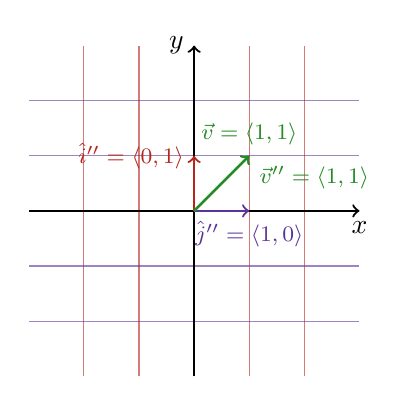
\begin{tikzpicture}[
        vector/.style={->, thick},
        scale=0.7
    ]

    \foreach \i in {-2, -1, ..., 2} {
        \draw[BrickRed, thin, opacity=0.6] (\i, -3) -- (\i, 3);
        \draw[RoyalPurple, thin, opacity=0.6] (-3, \i) -- (3, \i);
    }
    \draw[vector, black] (-3, 0) -- (3, 0) node[below] {$x$};
    \draw[vector, black] (0, -3) -- (0, 3) node[left] {$y$};

    \draw[vector, BrickRed] (0, 0) -- (0, 1)
        node[left, BrickRed]
            {\footnotesize $\hat{i}'' = \langle 0, 1 \rangle$};
    \draw[vector, RoyalPurple] (0, 0) -- (1, 0)
        node[below, RoyalPurple]
            {\footnotesize $\hat{j}'' = \langle 1, 0 \rangle$};
    \draw[vector, ForestGreen] (0, 0) -- (1, 1)
        node[above, dotted, ForestGreen]
            {\footnotesize $\vec{v} = \langle 1, 1 \rangle$};
    \draw[vector, ForestGreen] (0, 0) -- (1, 1)
        node[below right, ForestGreen]
            {\footnotesize $\vec{v}'' = \langle 1, 1 \rangle$};
\end{tikzpicture}
\end{figure}
\end{minipage}
\hfill
\begin{minipage}{0.48\textwidth}
\begin{figure}[H]
\centering
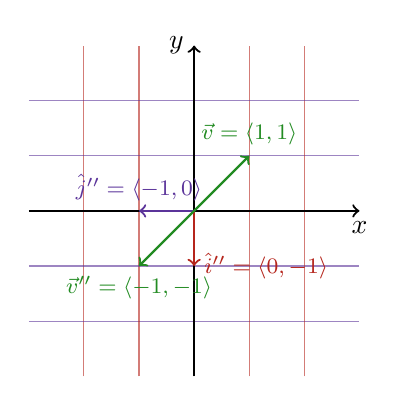
\begin{tikzpicture}[
        vector/.style={->, thick},
        scale=0.7
    ]

    \foreach \i in {-2, -1, ..., 2} {
        \draw[BrickRed, thin, opacity=0.6] (\i, -3) -- (\i, 3);
        \draw[RoyalPurple, thin, opacity=0.6] (-3, \i) -- (3, \i);
    }
    \draw[vector, black] (-3, 0) -- (3, 0) node[below] {$x$};
    \draw[vector, black] (0, -3) -- (0, 3) node[left] {$y$};

    \draw[vector, BrickRed] (0, 0) -- (0, -1)
        node[right, BrickRed]
            {\footnotesize $\hat{i}'' = \langle 0, -1 \rangle$};
    \draw[vector, RoyalPurple] (0, 0) -- (-1, 0)
        node[above, RoyalPurple]
            {\footnotesize $\hat{j}'' = \langle -1, 0 \rangle$};
    \draw[vector, ForestGreen] (0, 0) -- (1, 1)
        node[above, dotted, ForestGreen]
            {\footnotesize $\vec{v} = \langle 1, 1 \rangle$};
    \draw[vector, ForestGreen] (0, 0) -- (-1, -1)
        node[below, ForestGreen]
            {\footnotesize $\vec{v}'' = \langle -1, -1 \rangle$};
\end{tikzpicture}
\end{figure}
\end{minipage}

Let's take a look at what's happening here. $\vec{v}''$ in our
left diagram can be represented as the following.
\[
\vec{v}'' =
\begin{bmatrix}
    -1 & 0 \\
    0  & 1
\end{bmatrix}
\left(
\begin{bmatrix}
    0 & -1 \\
    1 & 0
\end{bmatrix}
\begin{bmatrix}
    1 \\
    1
\end{bmatrix}
\right)
\]
Notice that we have to write it in the order $B(A\vec{v})$ as we
would be performing $A$ first. We can think of it as reading it from
left to right just as we would read from left to right when
computing composite functions.
\[
\vec{v}'' =
\begin{bmatrix}
    -1 & 0 \\
    0  & 1
\end{bmatrix}
\left(
\begin{bmatrix}
    0 & -1 \\
    1 & 0
\end{bmatrix}
\begin{bmatrix}
    1 \\
    1
\end{bmatrix}
\right)
=
\begin{bmatrix}
    -1 & 0 \\
    0  & 1
\end{bmatrix}
\left(
\begin{bmatrix}
    -1 \\
    1
\end{bmatrix}
\right)
=
\begin{bmatrix}
    1 \\
    1
\end{bmatrix}
\]
This is exactly what we have for the left diagram. We could do
the same for the right side.
\[
\vec{v}'' =
\begin{bmatrix}
    0 & -1 \\
    1 & 0
\end{bmatrix}
\left(
\begin{bmatrix}
    -1 & 0 \\
    0  & 1
\end{bmatrix}
\begin{bmatrix}
    1 \\
    1
\end{bmatrix}
\right)
=
\begin{bmatrix}
    0 & -1 \\
    1 & 0
\end{bmatrix}
\left(
\begin{bmatrix}
    -1 \\
    1
\end{bmatrix}
\right)
=
\begin{bmatrix}
    -1 \\
    -1
\end{bmatrix}
\]
This is also supported! Alternatively, we could just compute
$AB$ and $BA$ to see what our ``final transformation is''.
\begin{align*}
    BA &=
    \begin{bmatrix}
        -1 & 0 \\
        0  & 1
    \end{bmatrix}
    \begin{bmatrix}
        0 & -1 \\
        1 & 0
    \end{bmatrix}
    =
    \begin{bmatrix}
        0 & 1 \\
        1 & 0
    \end{bmatrix} \\
    AB &=
    \begin{bmatrix}
        0 & -1 \\
        1 & 0
    \end{bmatrix}
    \begin{bmatrix}
        -1 & 0 \\
        0  & 1
    \end{bmatrix}
    =
    \begin{bmatrix}
        0  & -1 \\
        -1 & 0
    \end{bmatrix}
\end{align*}
Clearly, we could see that the mapping is different.

Another interesting property for matrices $A$, $B$, and $C$ is that
even if $AC = BC$, it does not necessarily mean that $A = B$.
Think about the case when $C$ is a zero matrix. Although matrix
multiplication is not commutative, the associative and distributive
property still applies.

\begin{theorem}{Properties of Matrix Multiplication}
For matrices $A$, $B$, and $C$, the following equations are true
given that the conditions for the addition and multiplication are met.
\begin{enumerate}
\item $A(BC) = (AB)C$
\item $A(B + C) = AB + AC$
\item $(B + C)A = BA + CA$
\item $\lambda(AB) = A(\lambda B)$
\end{enumerate}
\end{theorem}

Let's start by proving the associative property.
\begin{proof}
Let $A = [a_{ij}]_{m \times n}$, $B = [b_{ij}]_{n \times q}$,
and $C = [c_{ij}]_{q \times r}$. First, notice that the elements
of the product $BC$, or $D = [d_{ij}]_{n \times r}$ can be
represented as $d_{ij} = \sum_{k=1}^{q} b_{ik} c_{kj}$. Multiplying
it again with $[a_{ij}]$, the elements of the product
$E = [e_{ij}]_{m \times r}$ can be represented as the following.
\[
e_{ij}
= \sum_{s=1}^{n} a_{is} d_{sj}
= \sum_{s=1}^{n} \left(
    a_{is} \sum_{k=1}^{q} b_{sk} c_{kj}
\right)
= \sum_{s=1}^{n} \sum_{k=1}^{q} a_{is} b_{sk} c_{kj}
\]
Similarly, we could do the same for the right-hand side of the
equation. Note that the elements of the product $AB$, or
$D' = [d'_{ij}]_{m \times q}$ can be represented as
$d'_{ij} = \sum_{k=1}^{n} a_{ik} b_{kj}$. Continuing, the elements
in the final product $E' = [e'_{ij}]_{m \times r}$ can be written as
the following.
\begin{align*}
    e'_{ij}
    &= \sum_{s=1}^{q} d'_{is} c_{sj}
    = \sum_{s=1}^{q} \left(
        \left(\sum_{k=1}^{n} a_{ik} b_{ks} \right) c_{sj}
    \right)
    = \sum_{s=1}^{q} \sum_{k=1}^{n} a_{ik} b_{ks} c_{sj} \\
    &= \sum_{k=1}^{q} \sum_{s=1}^{n} a_{is} b_{sk} c_{kj}
    = \sum_{s=1}^{n} \sum_{k=1}^{q} a_{is} b_{sk} c_{kj}
    = e_{ij}
\end{align*}
Because $e_{ij} = e'_{ij}$ for all possible combinations,
$A(BC) = (AB)C$.
\end{proof}
\begin{thoughts}
You might wonder if we are allowed to say that the following equation
is true.
\[
\sum_{k=1}^{q} \sum_{s=1}^{n} a_{is} b_{sk} c_{kj}
= \sum_{s=1}^{n} \sum_{k=1}^{q} a_{is} b_{sk} c_{kj}
\]
When proving this property, I initially thought that my proof
contained an error and spent my time reading the proof over and
over again. This actually applies and visualizing it helped me.
This part is not rigorous, so I didn't include it in the proof
above, but you can think of rotating the entire summation by
$90^\circ$.
\[
\sum_{k=1}^{q} \sum_{s=1}^{n} a_{is} b_{sk} c_{kj}
=
\begin{array}{ccc}
    a_{i1}b_{11}c_{1j} & & a_{i1}b_{1q}c_{qj} \\
    \vdots & + \cdots + & \vdots \\
    a_{in}b_{n1}c_{1j} & & a_{in}b_{nq}c_{qj}
\end{array}
\]
Similarly, the second sum can be represented as the following.
\[
\sum_{s=1}^{n} \sum_{k=1}^{q} a_{is} b_{sk} c_{kj}
=
\begin{array}{ccc}
    a_{i1}b_{11}c_{1j} & & a_{in}b_{n1}c_{1j} \\
    \vdots & + \cdots + & \vdots \\
    a_{i1}b_{1q}c_{qj} & & a_{in}b_{nq}c_{qj}
\end{array}
\]
Now imagine you write the entire terms out, and rotate it
$90^\circ$. They are identical!
\end{thoughts}

Next, let's prove the first distributive law.

\begin{proof}
Let $A = [a_{ij}]_{m \times n}$, $B = [b_{ij}]_{n \times q}$,
and $C = [c_{ij}]_{n \times q}$. Consider the following equation.
\begin{align*}
    [a_{ij}] \left( [b_{ij}] + [c_{ij}] \right)
    &= [a_{ij}] [b_{ij} + c_{ij}]
    = \left[ \sum_{k=1}^{n} a_{ik} (b_{kj} + c_{kj}) \right] \\
    &= \left[
        \sum_{k=1}^{n} a_{ik} b_{kj} + \sum_{k=1}^{n} a_{ik} c_{kj}
    \right] \\
    &= \left[ \sum_{k=1}^{n} a_{ik} b_{kj} \right]
        + \left[ \sum_{k=1}^{n} a_{ik} c_{kj} \right] \\
    &= [a_{ij}] [b_{ij}] + [a_{ij}] [c_{ij}]
\end{align*}
Therefore, the distributive property $A(B + C) = AB + AC$ applies.
\end{proof}

We could prove the right distributive law in similar fashion.

\begin{proof}
Let $A = [a_{ij}]_{n \times q}$, $B = [b_{ij}]_{m \times n}$,
and $C = [c_{ij}]_{m \times n}$. Consider the following equation.
\begin{align*}
    \left( [b_{ij}] + [c_{ij}] \right) [a_{ij}]
    &= [b_{ij} + c_{ij}] [a_{ij}]
    = \left[ \sum_{k=1}^{n} (b_{ik} + c_{ik}) a_{kj} \right] \\
    &= \left[
        \sum_{k=1}^{n} b_{ik} a_{kj} + \sum_{k=1}^{n} c_{ik} a_{kj}
    \right] \\
    &= \left[ \sum_{k=1}^{n} b_{ik} a_{kj} \right]
        + \left[ \sum_{k=1}^{n} c_{ik} a_{kj} \right] \\
    &= [b_{ij}] [a_{ij}] + [c_{ij}] [a_{ij}]
\end{align*}
Thus, the right distributive property $(B + C)A = BA + CA$ holds.
\end{proof}

Finally, let's prove the fourth property.

\begin{proof}
Let $A = [a_{ij}]_{m \times n}$ and $B = [b_{ij}]_{n \times p}$.
Consider the following equation.
\[
\lambda (AB)
= \lambda \left[ \sum_{k = 1}^{n} a_{ik} b_{kj} \right]
= \left[ \sum_{k = 1}^{n} \lambda a_{ik} b_{kj} \right]
= \left[ \sum_{k = 1}^{n} a_{ik} (\lambda b_{kj}) \right]
= A(\lambda B)
\]
Thus, the fourth property holds.
\end{proof}

In addition to the visual implications of a matrix and its
multiplication above, matrix multiplication can be extended to
systems of equations. For instance, consider the following system
of equations.
\begin{align*}
    2x + 3y &= 5 \\
    -x + 7y &= 3
\end{align*}
Using \textbf{coefficient matrix}, we could represent the system
above as the following matrix multiplication.
\[
\begin{bmatrix}
    2  & 3 \\
    -1 & 7
\end{bmatrix}
\begin{bmatrix}
    x \\
    y
\end{bmatrix}
=
\begin{bmatrix}
    5 \\
    3
\end{bmatrix}
\]
Let's take a look at more interesting facts on matrix multiplication.

\begin{definition}
A square matrix with $1$ in all entries of its main diagonal and
$0$ in the other entries is an \textbf{identity matrix}, denoted as
$I_n$ for an identity matrix with order $n \times n$. Moreover,
all identity matrices satisfy the following equation for square
matrix $A$ that can be multiplied.
\[
AI = IA = A
\]
\end{definition}

This is called an identity matrix because when you multiply any
square matrix by the identity matrix with the corresponding order,
you get the square matrix itself. Consider the following examples.
\[
\begin{bmatrix}
    1 & 0 & 0 \\
    0 & 1 & 0 \\
    0 & 0 & 1
\end{bmatrix}
\begin{bmatrix}
    1 & 2 & 3 \\
    4 & 5 & 6 \\
    7 & 8 & 9
\end{bmatrix}
=
\begin{bmatrix}
    1 & 2 & 3 \\
    4 & 5 & 6 \\
    7 & 8 & 9
\end{bmatrix}
\]
From this, we can obtain an important fact about the uniqueness
of the identity matrix.

\begin{theorem}{Uniqueness of Identity Matrices}
The identity matrix $I$ for square matrices $A$ is unique.
\end{theorem}
\begin{proof}
For the sake of contradiction, let matrix $A_{m \times m}$ have two
unique identity matrices $I_{m \times m}$ and $J_{m \times m}$.
By definition, $AI = IA = A$ and $AJ = JA = A$. Therefore,
$AI = IA = AJ = JA$ and $AI = AJ$. Because $A$ is any square matrix
with order $m \times m$, let $A = I$. Substituting, $II = IJ$, and
$I = J$ is obtained by definition. By contradiction from the
assumption that $I \neq J$, the identity matrix for a square matrix
$A$ is unique.
\end{proof}

Another interesting insight on matrix multiplication is dissecting
the matrices being multiplied. Let's take a look at a simple example.
\begin{align*}
\begin{bmatrix}
    \scriptstyle a_{11} &
    \scriptstyle a_{12} &
    \scriptstyle a_{13} \\
    \scriptstyle a_{21} &
    \scriptstyle a_{22} &
    \scriptstyle a_{23}
\end{bmatrix}
&\begin{bmatrix}
    \scriptstyle b_{11} &
    \scriptstyle b_{12} \\
    \scriptstyle b_{21} &
    \scriptstyle b_{22} \\
    \scriptstyle b_{31} &
    \scriptstyle b_{32}
\end{bmatrix}
=
\begin{bmatrix}
    \scriptstyle a_{11} b_{11} + a_{12} b_{21} + a_{13} b_{31} &
    \scriptstyle a_{11} b_{12} + a_{12} b_{22} + a_{13} b_{32} \\
    \scriptstyle a_{21} b_{11} + a_{22} b_{21} + a_{23} b_{31} &
    \scriptstyle a_{21} b_{12} + a_{22} b_{22} + a_{23} b_{32}
\end{bmatrix} \\
&=
\begin{bmatrix}
    \scriptstyle a_{11} &
    \scriptstyle a_{12} &
    \scriptstyle a_{13} \\
    \scriptstyle 0      &
    \scriptstyle 0      &
    \scriptstyle 0
\end{bmatrix}
\begin{bmatrix}
    \scriptstyle b_{11} &
    \scriptstyle b_{12} \\
    \scriptstyle b_{21} &
    \scriptstyle b_{22} \\
    \scriptstyle b_{31} &
    \scriptstyle b_{32}
\end{bmatrix}
+
\begin{bmatrix}
    \scriptstyle 0      &
    \scriptstyle 0      &
    \scriptstyle 0 \\
    \scriptstyle a_{21} &
    \scriptstyle a_{22} &
    \scriptstyle a_{23}
\end{bmatrix}
\begin{bmatrix}
    \scriptstyle b_{11} & \scriptstyle b_{12} \\
    \scriptstyle b_{21} & \scriptstyle b_{22} \\
    \scriptstyle b_{31} & \scriptstyle b_{32}
\end{bmatrix} \\
&=
\begin{bmatrix}
    \scriptstyle a_{11} &
    \scriptstyle a_{12} &
    \scriptstyle a_{13} \\
    \scriptstyle a_{21} &
    \scriptstyle a_{22} &
    \scriptstyle a_{23}
\end{bmatrix}
\begin{bmatrix}
    \scriptstyle b_{11} & \scriptstyle 0 \\
    \scriptstyle b_{21} & \scriptstyle 0 \\
    \scriptstyle b_{31} & \scriptstyle 0
\end{bmatrix}
+
\begin{bmatrix}
    \scriptstyle a_{11} &
    \scriptstyle a_{12} &
    \scriptstyle a_{13} \\
    \scriptstyle a_{21} &
    \scriptstyle a_{22} &
    \scriptstyle a_{23}
\end{bmatrix}
\begin{bmatrix}
    \scriptstyle 0 & \scriptstyle b_{12} \\
    \scriptstyle 0 & \scriptstyle b_{22} \\
    \scriptstyle 0 & \scriptstyle b_{32}
\end{bmatrix}
\end{align*}
In the matrix multiplication above, we could see that to find
the element in the entry $(i, j)$, it is sufficient for us to
see row $i$ from the left matrix and column $j$ from the right.
In the next section of the note, we will discuss different
topics about matrix.

\section{Additional Fundamental Topics}

This section discusses frequently appearing concepts in matrices
that they have their own names!

\subsection{Transpose}

Let's begin with transpose of a matrix.

\begin{definition}
The \textbf{transpose} of a matrix $A$ is defined by a matrix that
has switched rows and columns of $A$, i.e. each element is defined
as following.
\[
(A^\intercal)_{ij} = A_{ji}
\]
\end{definition}

Let's take a look at an example. You could think of it as holding
the left top and bottom right of a matrix and rotating to see its
back. For matrix $A$ defined as the following,
\[
A =
\begin{bmatrix}
    1 & 2 & 3 & 4 \\
    5 & 6 & 7 & 8
\end{bmatrix}
\]
its transpose, or $A$ transpose is defined as the following.
\[
A^\intercal =
\begin{bmatrix}
    1 & 5 \\
    2 & 6 \\
    3 & 7 \\
    4 & 8
\end{bmatrix}
\]
As you can see, if $A$ has the order $m \times n$, its transpose
will have the order $n \times m$. Another observation that we can
make is that a transpose of a row matrix is a column matrix and
vice versa. Here is a quick example. Assume matrix $A$ defined
as the following.
\[
A =
\begin{bmatrix}
    1 & 2 & 3
\end{bmatrix}
\]
The transpose of $A$ can be represented as the following.
\[
A^\intercal =
\begin{bmatrix}
    1 \\
    2 \\
    3
\end{bmatrix}
\]
Notice that the transpose of transpose of $A$ is simply $A$.
\[
(A^\intercal)^\intercal =
\begin{bmatrix}
    1 & 2 & 3
\end{bmatrix}
= A
\]
Before formally stating our observations, here are few definitions
to note.

\begin{definition}
A positive integral powers of $A$, or multiplying the matrix $n$
times can be represented as $A^n$. $A^0$ is defined to be the
identity matrix $I_n$ with corresponding order $n$. A square
matrix is \textbf{nilpotent} if there exists $n \in \mathbb{Z}$
such that $A^n = 0$.
\end{definition}

Other definitions from transpose is symmetry and skew-symmetry.

\begin{definition}
For matrix $A$ and its transpose $A^\intercal$, matrix $A$ is
\textbf{symmetric} if $A^\intercal = A$ and \textbf{skew-symmetric}
if $A^\intercal = -A$.
\end{definition}

An example of a symmetric matrix is the identity matrix. For more
general example, matrix $A$ and $B$ below are symmetric and
skew-symmetric respectively.
\[
A =
\begin{bmatrix}
    a & b & c \\
    b & d & e \\
    c & e & f
\end{bmatrix},
\quad
B =
\begin{bmatrix}
    0  & a  & b \\
    -a & 0  & c \\
    -b & -c & 0
\end{bmatrix}
\]
Notice that all symmetric and skew-symmetric matrices are square
matrices. Moreover, the diagonal elements must be zero for a
square matrix to be skew-symmetric.

Now let's discuss the properties of transpose of a matrix.

\begin{theorem}{Properties of Transpose of a Matrix}
For matrix $A$, $B$, scalar $\lambda$ and positive integer $n$,
the following equations are true assuming that the addition and
multiplication conditions are satisfied.
\begin{enumerate}
\item $(A^\intercal)^\intercal = A$
\item $(A + B)^\intercal = A^\intercal + B^\intercal$
\item $(\lambda A)^\intercal = \lambda A^\intercal$
\item $(AB)^\intercal = B^\intercal A^\intercal$
\item $(A^n)^\intercal = (A^\intercal)^n$
\end{enumerate}
\end{theorem}

There are lots of properties to prove, but let's do them one by one.
Below is the proof for the first property.

\begin{proof}
Let $A = [a_{ij}]_{m \times n}$. By definition, its transpose
$A^\intercal \coloneqq [a_{ji}]_{n \times m}$. Continuing,
$\left( [a_{ji}]_{n \times m} \right)^\intercal =
[a_{ij}]_{m \times n} = A$. Therefore, $(A^\intercal)^\intercal = A$.
\end{proof}

Below is the proof for the second property.

\begin{proof}
Let $A = [a_{ij}]_{m \times n}$ and $B = [b_{ij}]_{m \times n}$.
Consider the following equation.
\begin{align*}
(A + B)^\intercal
&= \left(
    [a_{ij}]_{m \times n} + [b_{ij}]_{m \times n}
\right)^\intercal
= \left(
    [a_{ij} + b_{ij}]_{m \times n}
\right)^\intercal \\
&= [a_{ji} + b_{ji}]_{n \times m}
= [a_{ji}]_{n \times m} + [b_{ji}]_{n \times m} \\
&= A^\intercal + B^\intercal
\end{align*}
Thus, the property holds.
\end{proof}

Let's continue our proof for $(\lambda A)^\intercal =
\lambda A^\intercal$.

\begin{proof}
Let $A = [a_{ij}]_{m \times n}$. Because
$(\lambda A)^\intercal
= [\lambda a_{ij}]_{m \times n}^\intercal
= [\lambda a_{ji}]_{n \times m}
= \lambda [a_{ji}]_{n \times m}
= \lambda A^\intercal$, the property holds.
\end{proof}

We have two more left! Here is the proof for the fourth property.

\begin{proof}
Let $A = [a_{ij}]_{m \times n}$ and $B = [b_{ij}]_{n \times p}$.
The following equation is satisfied by definitions of matrix
multiplication and transpose.
\begin{align*}
    (AB)^\intercal
    &= \left(
        [a_{ij}]_{m \times n} [b_{ij}]_{n \times p}
    \right)^\intercal
    = \left(
        \left[ \sum_{k = 1}^{n} a_{ik} b_{kj} \right]_{m \times p}
    \right)^\intercal \\
    &= \left[ \sum_{k = 1}^{n} a_{jk} b_{ki} \right]_{p \times m}
\end{align*}
Continuing from the right hand side, the following equation is
obtained.
\begin{align*}
    B^\intercal A^\intercal
    &= \left[ b_{ij}^\intercal \right]_{p \times n}
        \left[ a_{ij}^\intercal \right]_{n \times m}
    = \left[
        \sum_{k = 1}^{n} b_{ik}^\intercal a_{kj}^\intercal
    \right]_{p \times m} \\
    &= \left[ \sum_{k = 1}^{n} b_{ki} a_{jk} \right]_{p \times m}
    = \left[ \sum_{k = 1}^{n} a_{jk} b_{ki} \right]_{p \times m}
\end{align*}
Because both the left-hand side and the right-hand side of the
equation lead to the same matrix, the property holds.
\end{proof}

Finally, below is the proof for the corollary of the fourth property.

\begin{proof}
First, notice that by the fourth property, the following equation
holds.
\[
\left( A^2 \right)^\intercal
= A^\intercal A^\intercal
= \left( A^\intercal \right)^2
\]
Therefore, it suffices to show that $(A^n)^\intercal =
(A^\intercal)^n$ holds for $n = k + 1$ if it is true for $n = k$.
Assume $(A^k)^\intercal = (A^\intercal)^k$. By the fourth property,
the following equation is obtained.
\[
\left( A^{k+1} \right)^\intercal
(A^k A)^\intercal
= (A^k)^\intercal A^\intercal
= (A^\intercal)^k A^\intercal
= (A^\intercal)^{k + 1}
\]
By induction, the property holds for $k \geq 2$. For $k = 1$,
it is self evident that the property holds true. Therefore, the
property holds for all positive integers $n$.
\end{proof}

For the next part of the section, we will discuss partitions.

\subsection{Partitions}

As always, let's start with key definitions.

\begin{definition}
As the name suggests a \textbf{submatrix} is a matrix of $A$ that
is obtained by omitting certain rows or columns.
\end{definition}

Consider matrix $A$ defined as the following.
\[
A =
\begin{bmatrix}
    1 & 2 & 3 \\
    4 & 5 & 6 \\
    7 & 8 & 9
\end{bmatrix}
\]
Below are a few example of submatrices of $A$.
\begin{align*}
A =
\begin{bmatrix}
    \tikzmarknode{a11}{1} &
    \tikzmarknode{a12}{2} &
    \tikzmarknode{a13}{3} \\
    \tikzmarknode{a21}{4} &
    \tikzmarknode{a22}{5} &
    \tikzmarknode{a23}{6} \\
    \tikzmarknode{a31}{7} &
    \tikzmarknode{a32}{8} &
    \tikzmarknode{a33}{9}
\end{bmatrix}
\begin{tikzpicture}[
        overlay, remember picture,
        arrow/.style = {-, very thick, opacity=0.7}
    ]
    \draw[arrow, Red] (a21.west)  -- (a23.east);
\end{tikzpicture}
&\rightarrow
\begin{bmatrix}
    1 & 2 & 3 \\
    7 & 8 & 9
\end{bmatrix} \\
A =
\begin{bmatrix}
    \tikzmarknode{a11}{1} &
    \tikzmarknode{a12}{2} &
    \tikzmarknode{a13}{3} \\
    \tikzmarknode{a21}{4} &
    \tikzmarknode{a22}{5} &
    \tikzmarknode{a23}{6} \\
    \tikzmarknode{a31}{7} &
    \tikzmarknode{a32}{8} &
    \tikzmarknode{a33}{9}
\end{bmatrix}
\begin{tikzpicture}[
        overlay, remember picture,
        arrow/.style = {-, very thick, opacity=0.7}
    ]
    \draw[arrow, Red] (a11.west) -- (a13.east);
    \draw[arrow, Red] (a31.west) -- (a33.east);
    \draw[arrow, Red] (a12.north) -- (a32.south);
\end{tikzpicture}
&\rightarrow
\begin{bmatrix}
    4 & 6
\end{bmatrix}
\end{align*}

\begin{definition}
We say the matrix is \textbf{partitioned} if horizontal and vertical
lines are used to divide the matrix into submatrices.
\end{definition}

Here are a few examples of different partitions of $A$.
\[
\begin{bNiceArray}{ccc}[margin]
    1 & 2 & 3 \\
    4 & 5 & 6 \\
    \hline
    7 & 8 & 9
\end{bNiceArray},
\quad
\begin{bNiceArray}{c|cc}[margin]
    1 & \textcolor{Red}{2} & \textcolor{Red}{3} \\
    4 & \textcolor{Red}{5} & \textcolor{Red}{6} \\
    \hline
    7 & 8 & 9
\end{bNiceArray},
\quad
\begin{bNiceArray}{c|c|c}[margin]
    1 & 2 & 3 \\
    \hline
    4 & 5 & 6 \\
    7 & 8 & 9
\end{bNiceArray}
\]
From different partitions, we can obtain different \textbf{blocks}.

\begin{definition}
A \textbf{block} of a partition of $A$ is a submatrix of $A$ divided
by the horizontal and vertical partition lines.
\end{definition}

The highlighted portion of the second partition above is an example
of a block. Now, why should we even care about partitions and blocks?
Partitions of a matrix are important because it could be a very
useful tool in computationally heavy matrix multiplication.
Let's take a look at a generalized example $AB$.
\[
AB =
\begin{bmatrix}
    a_{11} & a_{12} & a_{13} & a_{14} \\
    a_{21} & a_{22} & a_{23} & a_{24} \\
    a_{31} & a_{32} & a_{33} & a_{34} \\
    a_{41} & a_{42} & a_{43} & a_{44}
\end{bmatrix}
\begin{bmatrix}
    b_{11} & b_{12} & b_{13} \\
    b_{21} & b_{22} & b_{23} \\
    b_{31} & b_{32} & b_{33} \\
    b_{41} & b_{42} & b_{43}
\end{bmatrix}
\]
At least for me, this multiplication looks very painful. Fortunately,
using partitions, we can turn this monster into a baby monster.
\begin{align*}
AB
&=
\begin{bNiceArray}{cc|cc}[margin]
    a_{11} & a_{12} & a_{13} & a_{14} \\
    a_{21} & a_{22} & a_{23} & a_{24} \\
    a_{31} & a_{32} & a_{33} & a_{34} \\
    a_{41} & a_{42} & a_{43} & a_{44}
\end{bNiceArray}
\begin{bNiceArray}{ccc}[margin]
    b_{11} & b_{12} & b_{13} \\
    b_{21} & b_{22} & b_{23} \\
    \hline
    b_{31} & b_{32} & b_{33} \\
    b_{41} & b_{42} & b_{43}
\end{bNiceArray} \\
&=
\begin{bmatrix}
    a_{11} & a_{12} \\
    a_{21} & a_{22} \\
    a_{31} & a_{32} \\
    a_{41} & a_{42}
\end{bmatrix}
\begin{bmatrix}
    b_{11} & b_{12} & b_{13} \\
    b_{21} & b_{22} & b_{23}
\end{bmatrix}
+
\begin{bmatrix}
    a_{13} & a_{14} \\
    a_{23} & a_{24} \\
    a_{33} & a_{34} \\
    a_{43} & a_{44}
\end{bmatrix}
\begin{bmatrix}
    b_{31} & b_{32} & b_{33} \\
    b_{41} & b_{42} & b_{43}
\end{bmatrix} \\
&=
\begin{bmatrix}
    \scriptscriptstyle a_{11}b_{11} + a_{12}b_{21} &
    \scriptscriptstyle a_{11}b_{12} + a_{12}b_{22} &
    \scriptscriptstyle a_{11}b_{13} + a_{12}b_{23} \\
    \scriptscriptstyle a_{21}b_{11} + a_{22}b_{21} &
    \scriptscriptstyle a_{21}b_{12} + a_{22}b_{22} &
    \scriptscriptstyle a_{21}b_{13} + a_{22}b_{23} \\
    \scriptscriptstyle a_{31}b_{11} + a_{32}b_{21} &
    \scriptscriptstyle a_{31}b_{12} + a_{32}b_{22} &
    \scriptscriptstyle a_{31}b_{13} + a_{32}b_{23} \\
    \scriptscriptstyle a_{41}b_{11} + a_{42}b_{21} &
    \scriptscriptstyle a_{41}b_{12} + a_{42}b_{22} &
    \scriptscriptstyle a_{41}b_{13} + a_{42}b_{23}
\end{bmatrix} \\
&\qquad\qquad\qquad\qquad+
\begin{bmatrix}
    \scriptscriptstyle a_{13}b_{31} + a_{14}b_{41} &
    \scriptscriptstyle a_{13}b_{32} + a_{14}b_{42} &
    \scriptscriptstyle a_{13}b_{33} + a_{14}b_{43} \\
    \scriptscriptstyle a_{23}b_{31} + a_{24}b_{41} &
    \scriptscriptstyle a_{23}b_{32} + a_{24}b_{42} &
    \scriptscriptstyle a_{23}b_{33} + a_{24}b_{43} \\
    \scriptscriptstyle a_{33}b_{31} + a_{34}b_{41} &
    \scriptscriptstyle a_{33}b_{32} + a_{34}b_{42} &
    \scriptscriptstyle a_{33}b_{33} + a_{34}b_{43} \\
    \scriptscriptstyle a_{43}b_{31} + a_{44}b_{41} &
    \scriptscriptstyle a_{43}b_{32} + a_{44}b_{42} &
    \scriptscriptstyle a_{43}b_{33} + a_{44}b_{43}
\end{bmatrix} \\
&=
\begin{bmatrix}
    \scriptscriptstyle
    a_{11}b_{11} + a_{12}b_{21} + a_{13}b_{31} + a_{14}b_{41} &
    \scriptscriptstyle
    a_{11}b_{12} + a_{12}b_{22} + a_{13}b_{32} + a_{14}b_{42} &
    \scriptscriptstyle
    a_{11}b_{13} + a_{12}b_{23} + a_{13}b_{33} + a_{14}b_{43} \\
    \scriptscriptstyle
    a_{21}b_{11} + a_{22}b_{21} + a_{23}b_{31} + a_{24}b_{41} &
    \scriptscriptstyle
    a_{21}b_{12} + a_{22}b_{22} + a_{23}b_{32} + a_{24}b_{42} &
    \scriptscriptstyle
    a_{21}b_{13} + a_{22}b_{23} + a_{23}b_{33} + a_{24}b_{43} \\
    \scriptscriptstyle
    a_{31}b_{11} + a_{32}b_{21} + a_{33}b_{31} + a_{34}b_{41} &
    \scriptscriptstyle
    a_{31}b_{12} + a_{32}b_{22} + a_{33}b_{32} + a_{34}b_{42} &
    \scriptscriptstyle
    a_{31}b_{13} + a_{32}b_{23} + a_{33}b_{33} + a_{34}b_{43} \\
    \scriptscriptstyle
    a_{41}b_{11} + a_{42}b_{21} + a_{43}b_{31} + a_{44}b_{41} &
    \scriptscriptstyle
    a_{41}b_{12} + a_{42}b_{22} + a_{43}b_{32} + a_{44}b_{42} &
    \scriptscriptstyle
    a_{41}b_{13} + a_{42}b_{23} + a_{43}b_{33} + a_{44}b_{43}
\end{bmatrix}
\end{align*}

Well, this looks good to me! If the matrices being multiplied
have higher dimension, partitioning such matrices could help in
computation and reducing mistakes. Now that we have seen partitions
of matrices, we could derive special forms from the ideas.

\subsection{Special Forms of Matrix}

As always, let's build from definitions.

\begin{definition}
A \textbf{Symmetrically partitioned matrix} refers to a partitioned
matrix such that its arrangements of the blocks are diagonally
symmetric. The \textbf{diagonal blocks} are the blocks that pass
through the diagonal symmetry.
\end{definition}

We could also define matrices with diagonal blocks that are not
necessarily symmetrically partitioned.

\begin{definition}
A \textbf{block diagonal matrix} is a matrix with square diagonal
blocks and zero on the other entries.
\end{definition}

Below is the general form for square matrices $A_i$.
\[
A =
\begin{bmatrix}
    A_1    & 0      & \cdots & 0 \\
    0      & A_2    & \cdots & 0 \\
    \vdots & \vdots & \ddots & 0 \\
    0      & 0      & 0      & 0 \\
\end{bmatrix}
\]
Continuing, we could define rows and columns based on its elements.

\begin{definition}
\textbf{Zero rows} and \textbf{zero columns} are rows and columns
composed of zeros respectively.
\end{definition}

This definition is quite straightforward, and now that we have
basic terms in mind, let's discuss two forms from the definitions
above.

\begin{definition}
Matrix in \textbf{row echelon form (REF)} satisfies the conditions
below.
\begin{itemize}[noitemsep]
\item
All nonzero leading entry is $1$. (Side note here is that some
textbooks and lectures do not require the leading entry to be $1$,
but I actually would like to keep it this way as this is how I
initially learned it.)
\item
All nonzero leading entries in a nonzero row in a later row are to
the right of nonzero leading entries in previous rows.
\item
If there are both nonzero and zero rows, all zero rows must appear
after the nonzero rows above.
\end{itemize}

The leading entry of matrices in REF is known as a \textbf{pivot}.
Similarly, matrices in \textbf{reduced row echelon form (RREF)}
are matrices that satisfy the following conditions.
\begin{itemize}[noitemsep]
\item
All nonzero leading entries in a nonzero row is $1$.
\item
If there are both nonzero and zero rows, all zero rows must appear
after the nonzero rows above.
\item
All leading $1$s in the succeeding rows appear in a column after the
columns with previous leading $1$s.
\item
The leading $1$ must be the only nonzero element present in each
column if there exists such $1$.
\end{itemize}
\end{definition}

Below are examples of a matrices in REF and RREF respectively.
\[
\begin{bmatrix}
    1 & 2 & 3 & 4 \\
    0 & 0 & 1 & 2 \\
    0 & 0 & 0 & 1 \\
    0 & 0 & 0 & 0
\end{bmatrix},
\quad
\begin{bmatrix}
    1 & 0 & 2 & 0 \\
    0 & 1 & 2 & 0 \\
    0 & 0 & 0 & 1 \\
    0 & 0 & 0 & 0
\end{bmatrix}
\]
Matrices that follow these forms will be very useful when solving
linear systems of equations, but we will save that for the latter
notes. Now let's discuss about triangular matrices.

Triangular matrices are a special type of square matrices that is
determined by elements below the main diagonal. If all its
elements below the main diagonal are zeros, we call it an
\textbf{upper triangular} matrix. Similarly, if all elements above
the main diagonal are zeros, we call them \textbf{lower triangular}
matrices. For more formal statement, consider the following
definition.

\begin{definition}
A square matrix $A = [a_{ij}]$ is \textbf{upper triangular} if
$a_{ij} = 0 \, \forall \, i > j$. Similarly, the matrix is
\textbf{lower triangular} if $a_{ij} = 0 \, \forall \, i < j$.
\end{definition}

Let's take a look at an example. The left and right matrices below
are upper triangular and lower triangular matrices respectively.
\[
\begin{bmatrix}
    1 & 2 & 3 & 4 \\
    0 & 2 & 3 & 4 \\
    0 & 0 & 3 & 4 \\
    0 & 0 & 0 & 4
\end{bmatrix},
\quad
\begin{bmatrix}
    1 & 0 & 0 & 0 \\
    2 & 1 & 0 & 0 \\
    3 & 2 & 1 & 0 \\
    0 & 3 & 2 & 0
\end{bmatrix}
\]
Now that we have definitions of triangular matrices in mind,
we can discuss a theorem from such matrices.

\begin{theorem}{Property of Triangular Matrix Multiplication}
The product of two lower triangular matrices is a lower triangular
matrix, and the product of two upper triangular matrices is an upper
triangular matrix.
\end{theorem}
\begin{proof}
Let $A = [a_{ij}]_{n \times n}$ and $B = [b_{ij}]_{n \times n}$ be
lower triangular matrices. Consider the following equation for their
product matrix $C = [c_{ij}]_{n \times n}$.
\[
C
= \left[ \sum_{k = 1}^{n} a_{ik} b_{kj} \right]
= \left[
    \sum_{k = 1}^{j-1} a_{ik} b_{kj}
        + \sum_{k = j}^{n} a_{ik} b_{kj}
\right]
\]
From the expression, it suffices to show that $\sum_{k = 1}^{j-1}
a_{ik} b_{kj} + \sum_{k = j}^{n} a_{ik} b_{kj} \linebreak = 0$ for
$i < j$. Notice that by definition, $b_{kj} = 0$ for all $k = 1$ to
$k = j-1$. Similarly, $a_{ik} = 0$ for all integer $k \in [j, n]$.
Therefore, $c_{ij} = 0$ for all $i < j$, proving the first half of
the theorem.

Similarly, let $A' = [a'_{ij}]_{n \times n}$ and $B' =
[b'_{ij}]_{n \times n}$ be upper triangular matrices. The product
matrix $C'= [c'_{ij}]_{n \times n}$ can be represented as following.
\[
C'
= \left[ \sum_{k = 1}^{n} a'_{ik} b'_{kj} \right]
= \left[
    \sum_{k = 1}^{j-1} a'_{ik} b'_{kj}
        + \sum_{k = j}^{n} a'_{ik} b'_{kj}
\right]
\]
By definition, it is evident that $a'_{ik} = 0$ for integer $k
\in [1, j-1]$ and $b'_{kj} = 0$ for integer $k \in [j, n]$.
Therefore, for $i > j$, $c'_{ij} = 0$ and the theorem is true.
\end{proof}

This is it for different topics on fundamentals of matrices! I know
this note is quite long, but let's conclude our notes with the
discussion on determinants.

\section{Determinants}

Finally determinants! One of the most foundational concepts in linear
algebra is the determinant. Being one of the foundational concepts,
I also think it is a hard concept if the intuition is excluded in the
discussion due to its formula heavy nature.

As you could have noticed, a linear transformation does not only
change the position of the vectors. Consider the following diagram.

\begin{figure}[H]
\centering
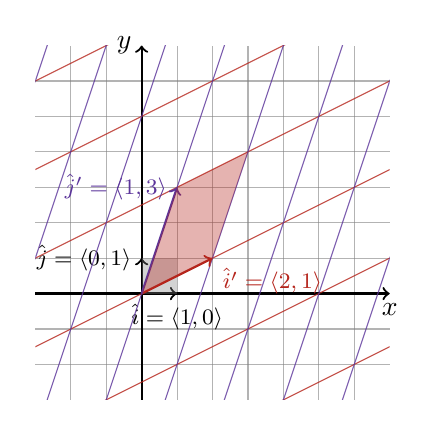
\begin{tikzpicture}[
        vector/.style={->, thick},
        scale=0.45
    ]

    \foreach \i in {-2, -1, ..., 6} {
        \draw[gray, thin, opacity=0.6] (\i, -3) -- (\i, 7);
        \draw[gray, thin, opacity=0.6] (-3, \i) -- (7, \i);
    }
    \draw[vector, black] (-3, 0) -- (7, 0) node[below] {$x$};
    \draw[vector, black] (0, -3) -- (0, 7) node[left] {$y$};

    \draw[vector] (0, 0) -- (1, 0) node[below]
        {\footnotesize $\hat{i} = \langle 1, 0 \rangle$};
    \draw[vector] (0, 0) -- (0, 1) node[left]
        {\footnotesize $\hat{j} = \langle 0, 1 \rangle$};
    \fill[Gray, opacity=0.35]
        (0,0) -- (1,0) -- (1,1) -- (0,1) -- cycle;

    \begin{scope}
        \clip (-3, -3) rectangle (7, 7);

        \foreach \j in {-10, -9, ..., 10} {
            \draw[BrickRed, opacity=0.8]
                ({-10*2 + \j*1}, {-10*1 + \j*3})
                    -- ({10*2 + \j*1}, {10*1 + \j*3});
        }
        \foreach \i in {-10, -9, ..., 10} {
            \draw[RoyalPurple, opacity=0.8]
                ({\i*2 + -10*1}, {\i*1 + -10*3})
                    -- ({\i*2 + 10*1}, {\i*1 + 10*3});
        }
    \end{scope}

    \draw[vector, BrickRed] (0, 0) -- (2, 1)
        node[below right, BrickRed]
            {\footnotesize $\hat{i}' = \langle 2, 1 \rangle$};
    \draw[vector, RoyalPurple] (0, 0) -- (1, 3)
        node[left, RoyalPurple]
            {\footnotesize $\hat{j}' = \langle 1, 3 \rangle$};
    \fill[BrickRed, opacity=0.35]
        (0,0) -- (2,1) -- (3,4) -- (1,3) -- cycle;
\end{tikzpicture}
\end{figure}

Notice that from the diagram above, the gray area is scaled to the
new red area. Notice that the area of the new parallelogram is
$3 \cdot 4 - 1 \cdot 2 \cdot \frac{1}{2} \cdot 2 - 1 \cdot 3 \cdot
\frac{1}{2} \cdot 2 - 1 \cdot 2 = 12 - 2 - 3 - 2 = 5$. Because
the area which was originally $1$ is scaled to $5$, we can say that
\[
\begin{vmatrix}
    2 & 1 \\
    1 & 3
\end{vmatrix}
= 5
\]
holds. The determinant is only defined for square matrices, and for
each square matrix, the determinants tell how much the area has
changed after the linear transformation. Determinants can surely
be negative, and they represent the change in orientation.
With this intuition in mind, let's discuss more computational
perspective of determinants.

Before we discuss the formula for determinants, let's define a
notation.

\begin{definition}
The \textbf{minor} of matrix $A$, denoted as $M_{ij}$, is a submatrix
of $A$ without the $i^\text{th}$ row and $j^\text{th}$ column of $A$.
The \textbf{cofactor} of $a_{ij}$ is defined as $(-1)^{i+j}
\det(M_{ij})$.
\end{definition}

Consider the following examples for $A$ defined as the following.
\[
A =
\begin{bmatrix}
    a_{11} & a_{12} & a_{13} & a_{14} \\
    a_{21} & a_{22} & a_{23} & a_{24} \\
    a_{31} & a_{32} & a_{33} & a_{34} \\
    a_{41} & a_{42} & a_{43} & a_{44}
\end{bmatrix}
\]
$M_{11}$ and $M_{24}$ are defined as the following.
\[
M_{11} =
\begin{bmatrix}
    a_{22} & a_{23} & a_{24} \\
    a_{32} & a_{33} & a_{34} \\
    a_{42} & a_{43} & a_{44}
\end{bmatrix}, \quad
M_{24} =
\begin{bmatrix}
    a_{11} & a_{12} & a_{13} \\
    a_{31} & a_{32} & a_{33} \\
    a_{41} & a_{42} & a_{43}
\end{bmatrix}
\]
Now let's define what determinants are with a recursive formula.

\begin{definition}
The \textbf{determinant} of a square matrix $A$, denoted as $\det(A)$
or $|A|$, is a value defined with the following rules.
\begin{enumerate}[noitemsep]
\item $\det(A) = a_{11}$ if $A = [a_{11}]$.
\item The following equation can be used to determine $\det(A)$ for
$A$ with order $n \times n$ for $n > 1$.
\vspace{-0.5\baselineskip}
\[
\det(A)
= \sum_{j=1}^n (-1)^{1 + j} a_{1j} \det(M_{1j})
\]
\end{enumerate}
\end{definition}

Let's take a look at an example with a $2 \times 2$ matrix
$A = [a_{ij}]$.
\begin{align*}
    \det(A)
    &= \sum_{j=1}^2 (-1)^{1 + j} a_{1j} \det(M_{1j}) \\
    &= (-1)^{1 + 1} a_{11} \det(M_{11}) +
        (-1)^{1 + 2} a_{12} \det(M_{12}) \\
    &= (-1)^{2} a_{11} a_{22} + (-1)^{3} a_{12} a_{21} \\
    &= a_{11} a_{22} - a_{12} a_{21}
\end{align*}
Returning to our first example, we can verify that the formula holds.
\[
\begin{vmatrix}
    2 & 1 \\
    1 & 3
\end{vmatrix}
= 2 \cdot 3 - 1 \cdot 1
= 5
\]
We could also derive the formula for higher orders with many
computations but I will leave them for you! I also think it is
just better to use the recursive formula and the formula for
$2 \times 2$ matrices instead of memorizing complex formulas,
but I don't know. I think it's up to you. Below is another
example.

\begin{align*}
    \det\left(
        \begin{bmatrix}
            1 & 0 & 0 \\
            0 & 1 & 0 \\
            0 & 0 & 1
        \end{bmatrix}
    \right)
    &= \sum_{j=1}^3 (-1)^{1 + j} a_{1j} \det(M_{1j}) \\
    &= a_{11} \det(M_{11})
    = 1 \cdot 1 - 0 \cdot 0 = 1
\end{align*}

With these in mind, we can establish a very important theorem in
computing determinants.

\begin{theorem}{Cofactor Expansion}
For any square matrix $A$, the cofactor expansion along the
$i^\text{th}$ row and the cofactor expansion along the $j^\text{th}$
column equal. In other words, the following equation holds.
\[
\det(A)
= \sum_{j=1}^n (-1)^{i + j} a_{ij} \det(M_{ij})
= \sum_{i=1}^n (-1)^{i + j} a_{ij} \det(M_{ij})
\]
\end{theorem}

Let's save the proof for the theorem for later as we need to show
different properties of determinants before proving the theorem
above. For now, let's discuss a special property of triangular
matrices.

\begin{theorem}{The Determinants of Triangular Matrices}
For a triangular (upper or lower) matrix $A_{n \times n} = [a_{ij}]$,
the determinant is defined as the following.
\[
\det(A)
= \prod_{i=1}^n a_{ii}
\]
\end{theorem}
\begin{proof}
First, the case for upper triangular matrix can be proven. Notice that
$\det(A) = \sum_{i=1}^n (-1)^{i + 1} a_{i1} \det(M_{i1}) =
a_{11} \det(M_{11})$ by Theorem \ref{theo:Cofactor Expansion}.
Continuing, notice that $M_{11}$ is another upper triangular matrix
by definition.

If such calculations are continued, it is evident that the last
term would be $a_{nn}$. Similarly, the second to the last term
would be $a_{nn} a_{n-1,n-1}$. By inductive hypothesis, it is
evident that
\[
\det(A)
= a_{11} \det(M_{11})
= a_{11} \prod_{i=2}^n a_{ii}
= \prod_{i=1}^n a_{ii}
\]
and the theorem holds for upper triangular matrix.

The case for lower triangular matrix can be proven in similar
manner. Note that $\det(A) = \sum_{j=1}^n (-1)^{1 + j} a_{1j}
\det(M_{1j}) = a_{11} \det(M_{11})$. With the same inductive
hypothesis above, it can be concluded that
\[
\det(A)
= a_{11} \det(M_{11})
= a_{11} \prod_{i=2}^n a_{ii}
= \prod_{i=1}^n a_{ii}
\]
and the theorem holds.
\end{proof}

As you could have guessed, we get a direct corollary from the
theorem.

\begin{corollary}{Determinants of Diagonal Matrices}
The determinant of any diagonal matrix is the product of the
diagonal entries.
\end{corollary}
\begin{proof}
First and foremost, notice that a diagonal matrix is both
an upper and lower triangular matrix. Thus by Theorem \ref{theo:The
Determinants of Triangular Matrices}, the corollary holds.
\end{proof}

Continuing from triangular matrices, we can also apply our
understanding of a transpose of a matrix. Consider the following
theorem.

\begin{theorem}{Transpose and Determinants}
$\det(A) = \det(A^\intercal)$ holds for all square matrix $A$.
\end{theorem}
\begin{proof}
First and foremost, notice that $A = A^\intercal$ if $A$ is a
$1 \times 1$ matrix. Thus, the theorem holds for any $A_{1 \times 1}$.
Continuing, note that for $A_{n \times n}$ with $n > 1$, $M_{ij}$
equals $M'_{ij}$ for $A^T$. Moreover by definition, $M'_{ij} =
M_{ji}$ and the following equation holds $A^\intercal = [a'_{ij}]$.
\begin{align*}
    \det(A)
    &= \sum_{i=1}^n (-1)^{i + 1} a_{i1} \det(M_{i1}) \\
    &= \sum_{j=1}^n (-1)^{1 + j} a'_{1j} \det(M'_{1j}) \\
    &= \det\left( A^\intercal \right)
\end{align*}
Thus, the theorem holds.
\end{proof}

Now that we discussed the relationships between matrices and
determinants, let's conclude our discussion with products and
determinants.

\subsection{Determinant and Products}

Before we conclude our discussion on determinant and this note,
I wished to introduce one of the most important results of
determinants. In this part of the section, we will try to prove
that the product of the determinants is the same as the determinant
of the product. To prove this result, we would need a lot of lemmas,
so let's get started with the first one.

\begin{lemma}{Determinants and Elementary Matrices I}
For a matrix $A_{n \times n}$ and an elementary matrix
$E_{n \times n}$ for interchanging two rows, $\det(E) = -1$
and $\det(EA) = \det(E) \det(A)$.
\end{lemma}
\begin{proof}
First and foremost, the case when $E$ exchanges two consecutive
rows can be proven. Let $B = FA$ where $F$ is the $n \times n$
elementary matrix that interchanges the $k^\text{th}$ and
$k+1^\text{th}$ rows of $A$. Therefore, for $A = [a_{ij}]$ and
$B = [b_{ij}]$, $b_{k+1,j} = a_{kj}$ holds and for the minor of $B$ as
$M'_{ij}$, $M'_{i+1,j} = M_{ij}$. Moreover, notice that $F = -1$ for
$n = 2$ and by inductive hypothesis with exchanging the use of
$\det(A) = (-1)^2 a_{11} \det(M_{11})$ and $\det(A) = (-1)^{2n} a_{nn}
\det(M_{nn})$, it is evident that $\det(F) = -1$. Thus, the following
equations hold.
\begin{align*}
    \det(B)
    &= \sum_{j=1}^n (-1)^{k+1+j} b_{k+1,j} \det(M'_{k+1,j}) \\
    &= \sum_{j=1}^n (-1)^{k+1+j} a_{kj} \det(M_{kj}) \\
    &= -\sum_{j=1}^n (-1)^{k+j} a_{kj} \det(M_{kj}) \\
    &= -\det(A)
\end{align*}
Thus, $\det(FA) = \det(F) \cdot \det(A)$. Continuing, notice that
any exchange between two consecutive rows requires one $F$. Moreover,
any exchange between two rows with a row in between requires three
$F$s. Since any exchange can be performed with the combination of
such two operations, it is evident that every $E$ can be represented
as odd number of $F$s. Therefore, the following equations hold for
odd $m$.
\begin{align*}
    \det(EA)
    &= \det(F_1 F_2 \cdots F_m A)
    = \det(F_1) \det(F_2) \cdots \det(F_m) \det(A) \\
    &= (-1)^m \det(A)
    = -\det(A) \\
    &= \det(E) \det(A)
\end{align*}
Thus, the lemma holds.
\end{proof}

Continuing from this lemma, we can establish an interesting corollary.

\begin{corollary}{Identical Rows or Columns and Determinant}
The equation $\det(A) = 0$ holds for all square matrices $A$ with
either two identical rows or columns.
\end{corollary}
\begin{proof}
Let $k_1$ and $k_2$ be the identical rows of the matrix $A$.
For an elementary matrix $E$ that interchanges the rows $k_1$ and
$k_2$, the following equations hold by Lemma \ref{lem:Determinants
and Elementary Matrices I}.
\[
\det(A)
= \det(EA)
= \det(E) \det(A)
= -\det(A)
\]
Thus, $\det(A) = 0$. Similarly, if $A$ has two identical columns
$k_1$ and $k_2$, the same argument applies by Theorem
\ref{theo:Transpose and Determinants} as $\det(A) =
\det(A^\intercal)$.
\end{proof}

For our second lemma, we have another elementary row operation.

\begin{lemma}{Determinants and Elementary Matrices II}
For a matrix $A_{n \times n}$ and an elementary matrix
$E_{n \times n}$ that scales $k^\text{th}$ row of $A$ by some nonzero
scalar $\lambda$, $\det(E) = \lambda$ and $\det(EA) = \det(E)
\det(A)$.
\end{lemma}
\begin{proof}
First and foremost, because $E_{n \times n} = k$, it is evident
that utilizing $\det(A) = (-1)^2 a_{11} \det(M_{11})$ and $\det(A) =
(-1)^{2n} a_{nn} \det(M_{nn})$, appropriately will lead to $\det(E) =
\lambda$ with inductive hypothesis. Moreover, consider the following
equations.
\begin{align*}
    \det(EA)
    &= \sum_{i=1}^n (-1)^{1+k} \lambda a_{ik} \det(M_{ik}) \\
    &= \lambda \sum_{i=1}^n (-1)^{1+k} a_{ik} \det(M_{ik}) \\
    &= \lambda \det(A) = \det(E) \det(A)
\end{align*}
Thus, the lemma holds.
\end{proof}

Just like our first lemma, we can expand this second lemma with
an interesting corollary.

\begin{corollary}{Scalars and Determinants}
For any matrix $A_{n \times n}$ and scalars $\lambda$,
$\det(\lambda A) = \lambda^n \det(A)$.
\end{corollary}
\begin{proof}
Let $E_k$ be the elementary row operation that scales the
$k^\text{th}$ row of $A$ by $\lambda$. Then, the following equations
hold by Lemma \ref{lem:Determinants and Elementary Matrices II}.
\begin{align*}
    \det(\lambda A)
    &= \det( E_n E_{n-1} \cdots E_1 A) \\
    &= \det(E_n) \det(E_{n-1}) \cdots \det(E_1) \det(A) \\
    &= \lambda^n \det(A)
\end{align*}
Thus, the corollary holds.
\end{proof}

Below is the third lemma on determinants and elementary matrices.

\begin{lemma}{Determinants and Elementary Matrices III}
For a matrix $A_{n \times n}$ and an elementary matrix $E$ of
the same order that adds $\lambda$ times row $k_1$ to row $k_2$
of $A$, then $\det(E) = 1$ and $\det(EA) = \det(E) \det(A)$.
\end{lemma}
\begin{proof}
First and foremost, notice that $E$ is a triangular matrix and
the elements in its diagonal are all $1$. Thus by Theorem
\ref{theo:The Determinants of Triangular Matrices}, $\det(E) = 1$.

Consider a new matrix $B$ that is obtained by replacing $k_2$
with $k_1$ from $A$. Then, $b_{k_2j} = a_{k_1j}$ and the minor
$M'_{ij}$ of $B$ satisfy $M'_{k_2j} = M_{k_2j}$. Moreover by Corollary
\ref{cor:Identical Rows or Columns and Determinant}, $\det(B) = 0$.
Therefore, the following equations hold.
\begin{align*}
    &\quad\ \det(EA) \\
    &= \sum_{j=1}^n (-1)^{k_2 + j} (a_{k_2j} + \lambda a_{k_1j})
        \det(M_{k_2j}) \\
    &= \sum_{j=1}^n (-1)^{k_2 + j} (a_{k_2j}) \det(M_{k_2j}) +
        \lambda \sum_{j=1}^n (-1)^{k_2 + j} (a_{k_1j})
            \det(M_{k_2j}) \\
    &= \det(A) + \lambda \det(B)
    = \det(A)
\end{align*}
Thus $\det(EA) = \det(A) = \det(E) \det(A)$.
\end{proof}

With the three lemmas above, we can establish an important theorem
that links the determinants of a matrix and an elementary matrix.

\begin{theorem}{Elementary Matrices and Determinants}
For a matrix $A_{n \times n}$ and any elementary matrix $E$ of the
same order, $\det(EA) = \det(E) \det(A)$.
\end{theorem}
\begin{proof}
By definition, there exists three different elementary matrices that
interchanges rows, scales a row, or add a scaled row to the other.
By Lemmas \ref{lem:Determinants and Elementary Matrices I},
\ref{lem:Determinants and Elementary Matrices II}, and
\ref{lem:Determinants and Elementary Matrices III}, $\det(EA) =
\det(E) \det(A)$ for all elementary matrices $E$.
\end{proof}

Now, I know it's lots of statements, but I promise we will get to
the main result. Let's take a look at one last important result to
get to our desired theorem! This theorem and its result include
the topic of invertibility, which has not been introduced yet. Please
feel free to read Section 3.3 and return or vice versa as it shouldn't
be something too hard.

\begin{theorem}{Invertibility and the Determinant}
A square matrix $A$ is invertible if and only if $\det(A) \neq 0$.
\end{theorem}
\begin{proof}
First, notice that $A$ is invertible if and only if there exists a
sequence of elementary matrices $E_1, \ldots, E_k$ such that
$E_k \cdots E_1 A = U$ holds for some upper triangular matrix $A$.
In other words,
\[
\det(E_k) \cdots \det(E_1) \det(A) = \det(U)
\]
where $\det(E_i) \neq 0$ and $\det(U) \neq 0$. Moreover, there exists
such elementary matrices if and only if $\det(A) \neq 0$. Thus, the
theorem holds.
\end{proof}

Now finally! Let's prove the theorem!

\begin{theorem}{Product and Determinants}
For square matrices $A$ and $B$ with the same order, $\det(AB) =
\det(A) \det(B)$.
\end{theorem}
\begin{proof}
First, the theorem can be shown for the case where $A$ is not
invertible. Notice that if $A$ is not invertible, then $AB$
must also be not invertible as if $AB$ is invertible, then
there exists a matrix $C$ such that $(AB)C = I$ and $A(BC) = I$,
which is contradictory. Thus by Theorem \ref{theo:Invertibility and
the Determinant}, $\det(AB) = 0 = 0 \cdot \det(B) = \det(A) \det(B)$
and the theorem holds for not invertible $A$.

Continuing, the case for invertible $A$ can be proven. By definition,
if $A$ is invertible, then it can be represented as a product of
sequence of elementary matrices $E_1, \ldots, E_k$. Therefore,
$\det(AB) = \det(E_1 \cdots E_k B) = \det(E_1 \cdots E_k) \det(B) =
\det(A) \det(B)$ by Theorem \ref{theo:Elementary Matrices and
Determinants}. Thus, the theorem holds.
\end{proof}

With this important theorem in mind, let's wrap up our notes with
two corollaries.

\begin{corollary}{Corollary of Product and Determinants I}
For an invertible matrix $A$, $\det(A^{-1}) = \frac{1}{\det(A)}$.
\end{corollary}
\begin{proof}
Notice that $1 = \det(AA^{-1}) = \det(A) \det(A^{-1})$ by Theorem
\ref{theo:Product and Determinants}. Therefore, $\det(A^{-1}) =
\frac{1}{\det(A)}$.
\end{proof}

Continuing, below is the second corollary.

\begin{corollary}{Corollary of Product and Determinants II}
If two matrices $A$ and $B$ are similar, then $\det(A) = \det(B)$.
\end{corollary}
\begin{proof}
By definition, if $A$ and $B$ are similar, then there exists an
invertible matrix $P$ that satisfy $A = P^{-1} B P$. Therefore
by Theorem \ref{theo:Product and Determinants} and Corollary
\ref{cor:Corollary of Product and Determinants I}, $\det(A) =
\det(P^{-1}) \det(B) \det(P) = \frac{1}{\det(P)} \cdot \det(B) \det(P)
= \det(B)$ and the corollary holds.
\end{proof}

This is it for determinants! I think it is an interesting way to
connect the relationship between linear transformations, which
we will discuss in future notes and matrix representation of their
effects. In the next notes, we will discuss different applications
of matrices.

\section{Practice Problems}
\begin{enumerate}
\item
Consider matrices $A$ and $B$ defined as the following.
\[
A =
\begin{bmatrix}
    1 & 2 \\
    2 & 0
\end{bmatrix},
\quad
B =
\begin{bmatrix}
    -1 & 2 \\
    0  & 3
\end{bmatrix}
\]
Compute the following matrix operations.
\begin{enumerate}[noitemsep]
\item $A - 2B$
\item $AB$
\item $(AB - BA)^\intercal$
\end{enumerate}

\item
Find $a_2B$ if $AB$ is defined as the following.
\[
AB =
\begin{bmatrix}
    1 & 2 & 3 \\
    4 & 5 & 6 \\
    7 & 8 & 9
\end{bmatrix}
\]

\item
Find matrix $A$ such that the following equation holds.
\[
2A - 3A^\intercal =
\begin{bmatrix}
    -1 & -5 \\
    0  & -4
\end{bmatrix}
\]

\item
Show that all square matrices can be represented as the sum of
symmetric and skew-symmetric matrices.

\item
Show that if $AB = BA$ for nilpotent matrices $A$ and $B$, then the
product $AB$ is nilpotent.

\item
Show that for square matrices $A$ and $B$, $AB + (AB)^\intercal$
is symmetric.

\item
For square matrices $A$ and $B$ of order $n \times n$, show that
the following equation holds \cite{refbook1}.
\[
\det\left(
    \begin{bmatrix}
        A & B \\
        B & A
    \end{bmatrix}
\right)
= \det(A + B) \det(A - B)
\]

\item
Show that if a square matrix $A$ is skew-symmetric, then $A^3$ is
also skew-symmetric.
\end{enumerate}
\end{document}


